\documentclass[11pt]{scrreprt}
\usepackage{dominatrix}
\usepackage{solarized-light}
\lstset{
language=R,
basicstyle=\ttfamily\tiny
}

\usepackage[toc,page]{appendix}
\usepackage{rotating}

\def\signed #1{{\leavevmode\unskip\nobreak\hfil\penalty50\hskip2em
  \hbox{}\nobreak\hfil(#1)%
  \parfillskip=0pt \finalhyphendemerits=0 \endgraf}}

\newsavebox\mybox
\newenvironment{aquote}[1]
  {\savebox\mybox{#1}\begin{quote}}
  {\signed{\usebox\mybox}\end{quote}}

\title{Principal Component Analysis of Interest Rate Swaps}
\subject{STAT W4290 Statistical Methods in Finance Final Project}
\author{Linan Qiu\\\texttt{lq2137@columbia.edu}}
\begin{document}
\maketitle

\setcounter{tocdepth}{1}
\tableofcontents

\begin{abstract}
This project applies Principal Component Analysis (PCA) to interest rate swaps and shows that the first 3 principal components correspond to yields, slope, and curvature respectively. I first start with vanilla interest rate swaps, and explain how an analysis based purely on single trades are unsatisfactory. I then shift our analysis to curve trades done using pairs of interest rate swaps and show how that is more useful in modeling different parts of the yield curve. I then demonstrate how the principal components from the analysis corresponding to yield, slope and curvature. Finally, I conclude by suggesting applications of this methodology in constructing better hedge ratios for interest rate swap pair trades than using pure duration analysis.
\end{abstract}

\chapter{Introduction and Background}
\section{Interest Rate Swaps}

Interest Rate Swaps (IRS) are increasingly important as a benchmark setting instrument and a speculation vehicle. It is an instrument in which two parties agree to exchange interest rate cash flows, based on a specified notional amount from a fixed rate to a floating rate. A detailed introduction to IRS is provided in the appendix.

\section{Speculation using Interest Rate Swaps}
A speculator that takes the "pay fixed" position on an 5 year IRS experiences the following cashflow:

\begin{itemize}
\item Pay fixed for 5 years, hence pays a fixed percentage of the notional amount every 6 months for 5 years. The rate paid is known as the \textbf{swap rate}.
\item Receive floating for 5 years, hence receives a floating percentage of the notional amount every 6 months based on the then spot LIBOR rate at the start of the 6 months. This goes on for 5 years as well.
\end{itemize}

This position profits if rates go up, since the speculator will be paying the same amount for a larger cashflow. Since the IRS has an initial value of zero, the swap rate is the discount factor that makes the present value of the fixed leg equal to the present value of the floating leg. Since the floating leg is discounted using the forward rates, the swap rate can be seen as an "average" of the forward rates up to 5 years.

One can use IRS to trade on the level of the forward curve, the slope of the forward curve, and the curvature of the forward curve. The details of these trades are explained in the appendix.

\chapter{Data}

\section{Data Source}

Data is collected from St. Louis Fed's FRED using the \texttt{quantmod} library in \texttt{R}. Specifically, I collected data for 1 year, 2 year, 3 year, 4 year, 5 year, 7 year, 10 year, and 30 year IRS swap rates. This data is used directly in the section dealing with PCA of IRS swap rates. In the section dealing with PCA of curve rates, the difference of different permutations of pairs of these rates are used to construct the curve rates. A total of \textbf{250} daily yields for the year to date (13 December 2015) are taken for each tenor.

\section{Eliminating Autocorrelation}

Level yields are highly autocorrelated as shown in Figure \ref{fig:acf-yields}. Despite the industry norm of using yield levels for PCA analysis, this is problematic for PCA which assumes that the input data is not autocorrelated.

\begin{table}[ht]
\centering
\begin{tabu}{r c c}
  \toprule
Lag & Level Rates & Percentage Change Rates \\ 
  \midrule
1 & 1.00 & 1.00 \\ 
  2 & 1.00 & -0.00 \\ 
  3 & 1.00 & -0.04 \\ 
  4 & 0.99 & -0.01 \\ 
  5 & 0.99 & -0.00 \\
   \bottomrule
\end{tabu}
\caption{Autocorrelation of Level Rates and Percentage Change of Rates using 7 Year IRS Swap Rates}
\label{table:autocorrelation}
\end{table}

Hence, I use the percentage change of yield rates instead to solve this problem resulting in much lower autocorrelation as shown in Figure \ref{fig:acf-yields-returns}.

\section{Principal Component Analysis}

PCA is performed on the \textbf{covariance} matrix of the percentage change of rates of each of the time series using the \texttt{princomp} package in \texttt{R}.

\chapter{PCA on IRS Level Trades}

\section{PCA Results}

\begin{figure}[H]
\begin{subfigure}{.3\textwidth}
\centering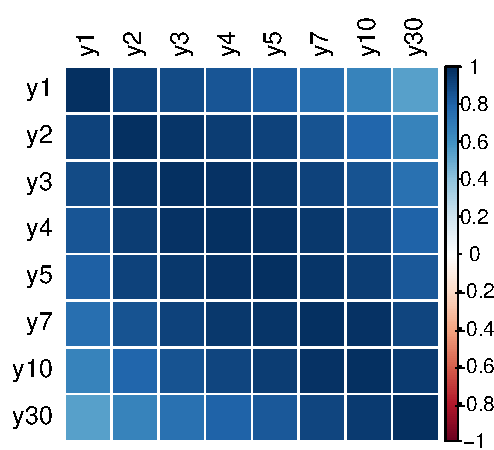
\includegraphics[]{corrplot-vanilla-returns.pdf}
\caption{Correlation of returns of rates}
\end{subfigure}
\begin{subfigure}{.3\textwidth}
\centering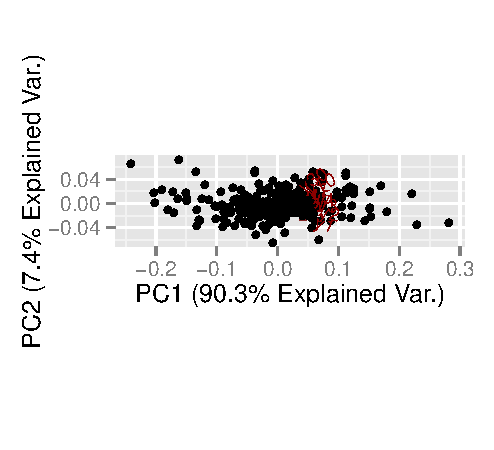
\includegraphics[]{biplot-vanilla-returns.pdf}
\caption{Biplot of first 2 principal components}
\end{subfigure}
\begin{subfigure}{.3\textwidth}
\centering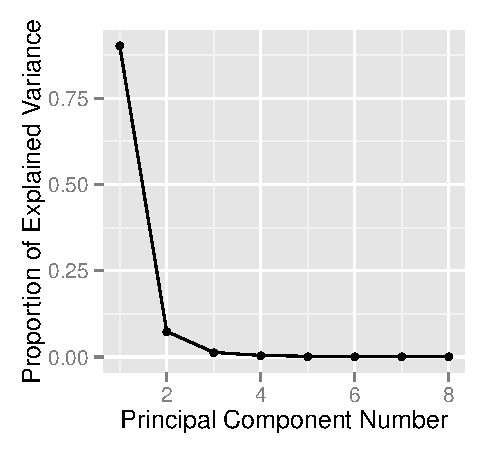
\includegraphics[]{screeplot-vanilla-returns.pdf}
\caption{Screeplot of principal components showing proportion of explained variance}
\end{subfigure}
\caption{Descriptive data for the input of PCA.}
\label{fig:descriptive-pca-vanilla}
\end{figure}

The data has a high degree of covariance among the time series. This should not be surprising at all, since the short end of the curve was included in all these measurements. Hence, in terms of dimensionality reduction, the first 3 principal components are representative of the data.

\section{Interpretation of Loadings}

However, I am also interested in the interpretation of the principal components. I hypothesized that the first 3 principal components should correspond to:

\begin{itemize}
\item PC1: Directional movements in the yield curve. These are movements that shift the entire yield curve up or down.
\item PC2: Slope movements in the yield curve. These are movements that steepen or flatten (change the first derivative wrt maturity) the entire yield curve.
\item PC3: Curvature movements in the yield curve. These are movements that change the curvature (or the second derivative wrt maturity) of the entire yield curve.
\end{itemize}

I find that this interpretation stands. By evaluating the loadings of the principal components shown in Table \ref{table:pca-loadings-level}, I observe that

\begin{itemize}
\item PC1: All IRS yields are weighted in the same direction (negative). Since the sign of the loadings are arbitrary, this means that PC1 reflects movements that causes IRS of all maturities to move in the same direction. This corresponds to directional movements in the yield curve -- if the yield curve goes up, all yields go up be it the short end or the long end and vice versa.
\item PC2: IRS yields on the short end of the curve (from y1 to y7) are weighted negatively and the ones reaching the long end (y10 and y30) are weighted positively. Since the signs are arbitrary, this means that PC2 reflects movements that cause the short end to go in one direction and the long end in the other. This is exactly what slope movements do -- if the yield curve steepens, the short end goes down and the long end goes up and vice versa if the yield curve flattens.
\item PC3: IRS yields on the short and long ends of the curve are weighted positively while the ones in the middle are weighted negatively. Since the signs are arbitrary, this means that PC3 reflects movements that cause the short and long end to go in one direction, and the middle to go in the other. This is exactly what curvature movements do -- if the yield curve increases in curvature, the short and long end goes down while the middle goes up.
\end{itemize}

Hence PC1 can be interpreted as directional movements, PC2 as slope movements, and PC3 as curvature movements. The scores for the PCA can be found in Figure \ref{fig:pca-scores-vanilla.pdf}.

\section{Drawbacks of Analysis}

I find this analysis lacking in one striking way: we are unable to isolate portions of the curve. For example, the time series for y30 includes movements from the spot all the way to year 30. In other words, it includes movements of the y1, y2, y3 etc. In a similar way, the y3 includes movements of y1. Hence, we are unable to isolate movements in the "long end only" and are instead forced to make conclusions about yield rates "from the short end to the long end" or on the "short end" only.

This could be done instead by measuring yields for curve trades. This is what I will do in the next section.

\chapter{PCA on IRS Curve Trades}

\section{Construction of Curve Yields}

The yield of a curve trade is calculated as follow:

\[C_{t_1, t_2} = S_{0, t_2} - S_{0, t_1}\]

where $C$ is the curve trade rate, $S_{0,t_2}$ is the swap rate for an IRS of maturity $t_2$ and $S_{0, t_2}$ is the swap rate for an IRS of maturity $t_1$. Intuitively, we can think of this the forward rate from $t_1$ to $t_2$ and indeed it is. I select the following "tenors" (sections of the yield curve) to represent the whole yield curve: 2s1s, 3s1s, 4s1s, 5s1s, 7s1s, 10s2s, 10s5s, 30s10s. They are quoted as "XsYs" where we pay fix for X years and receive fix for Y years of IRS. The same process for eliminating autocorrelation is done, so \textbf{returns on rates is used instead of level rates} as shown in Figure \ref{fig:acf-curve} and Figure \ref{fig:acf-curve-returns}. The curve rates extracted are shown in Figure \ref{fig:descriptive-curve-rates} and the returns on these rates are shown in \ref{fig:descriptive-curve-rates-returns}

\section{PCA Results}

\begin{figure}[H]
\begin{subfigure}{.3\textwidth}
\centering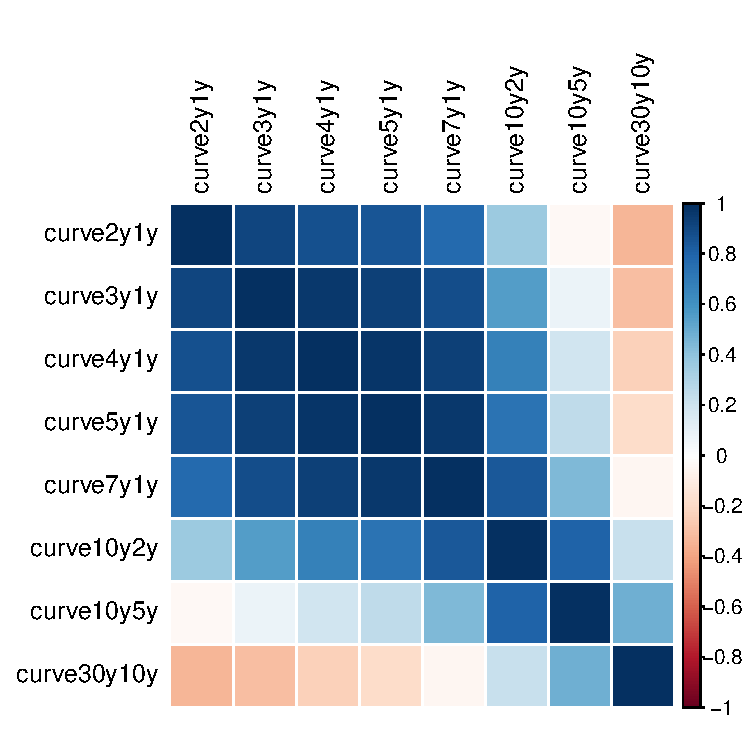
\includegraphics[]{corrplot-curve-returns.pdf}
\caption{Correlation of returns of rates}
\end{subfigure}
\begin{subfigure}{.3\textwidth}
\centering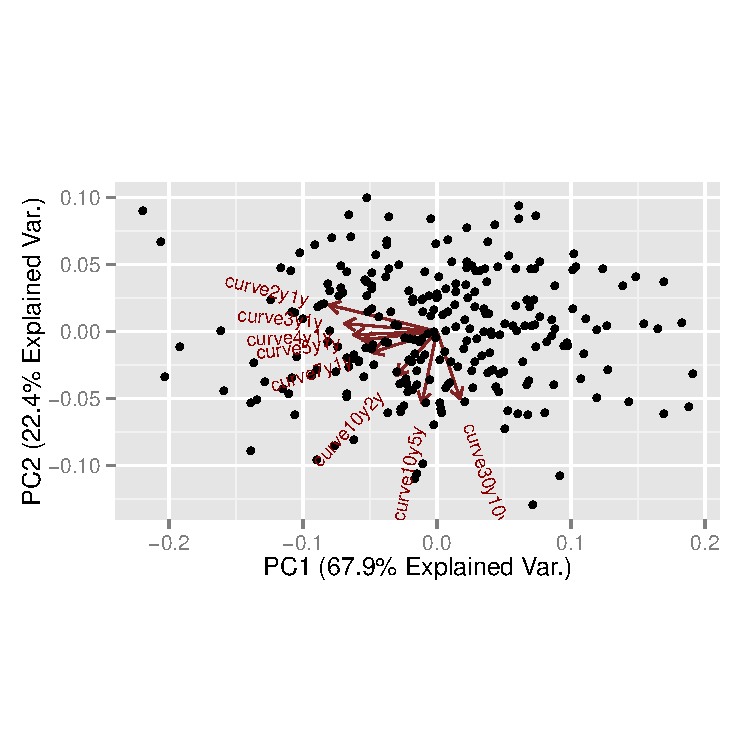
\includegraphics[]{biplot-curve-returns.pdf}
\caption{Biplot of first 2 principal components}
\end{subfigure}
\begin{subfigure}{.3\textwidth}
\centering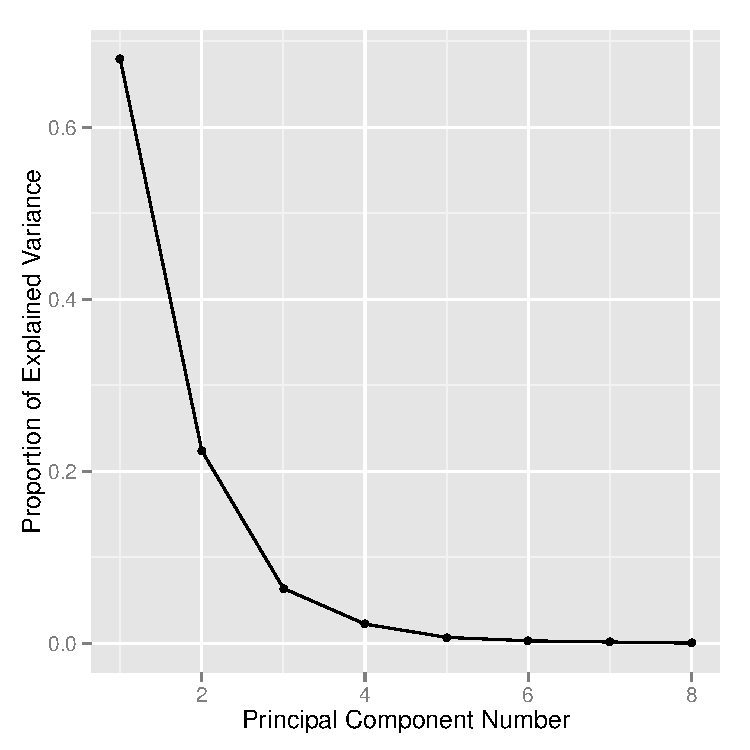
\includegraphics[]{screeplot-curve-returns.pdf}
\caption{Screeplot of principal components showing proportion of explained variance}
\end{subfigure}
\caption{Descriptive data for the input of PCA.}
\label{fig:descriptive-pca-curve}
\end{figure}

Again, the series has a high degree of covariance among the time series. This again should not be surprising, since they are all yield rates after all (though of different tenors) hence should be driven by the same macroeconomic factors. However, what should be interesting to note is that some time series now have somewhat negative covariance with others. These happen to be between the far short end of the curve and the far long end (eg. 2s1s vs 30s10s). This makes sense, since the far end usually doesn't move as much as the short end, and sometimes in the opposite direction (slope).

Again, the dimensionality reduction is successful, with the first 3 principal components accounting for 96.7\% of the variance (PC1: 67.9\%, PC2: 22.4\% and PC3: 6.4\%). The full table of explained variance is listed in \ref{fig:verbatim-curve}

\section{Interpretation of Loadings}

\begin{itemize}
\item Principal Component 1: Almost all the loadings are negative. Hence, in PC1 type movement, most sections of the yield curve move in the same direction (with the exception of the far end which moves in the opposite direction weakly). This corresponds to directional movements in the yield curve where the entire curve shifts up or down.
\item Principal Component 2: The short end of the curve (2s1s, 3s1s, 4s1s, 5s1s) are positive while the middle (7s1s, 10s2s, 10s5s) are negative as far the far end (30s10s). Again, signs are arbitrary in PCA loadings. This means that in PC2 type movements, the far and middle end moves in opposite direction as the short end. This corresponds well with the slope interpretation.
\item Principal Component 3: The short end and the long end moves in the same direction while the middle end moves in the opposite direction. This again corresponds well with the interpretation of curvature movements.
\end{itemize}

This relationship is summarized in the plot at Figure \ref{fig:pca-loadings-curve}.

\section{Verification of Interpretation of Loadings}

\subsection{First Factor}

\begin{figure}[H]
\centering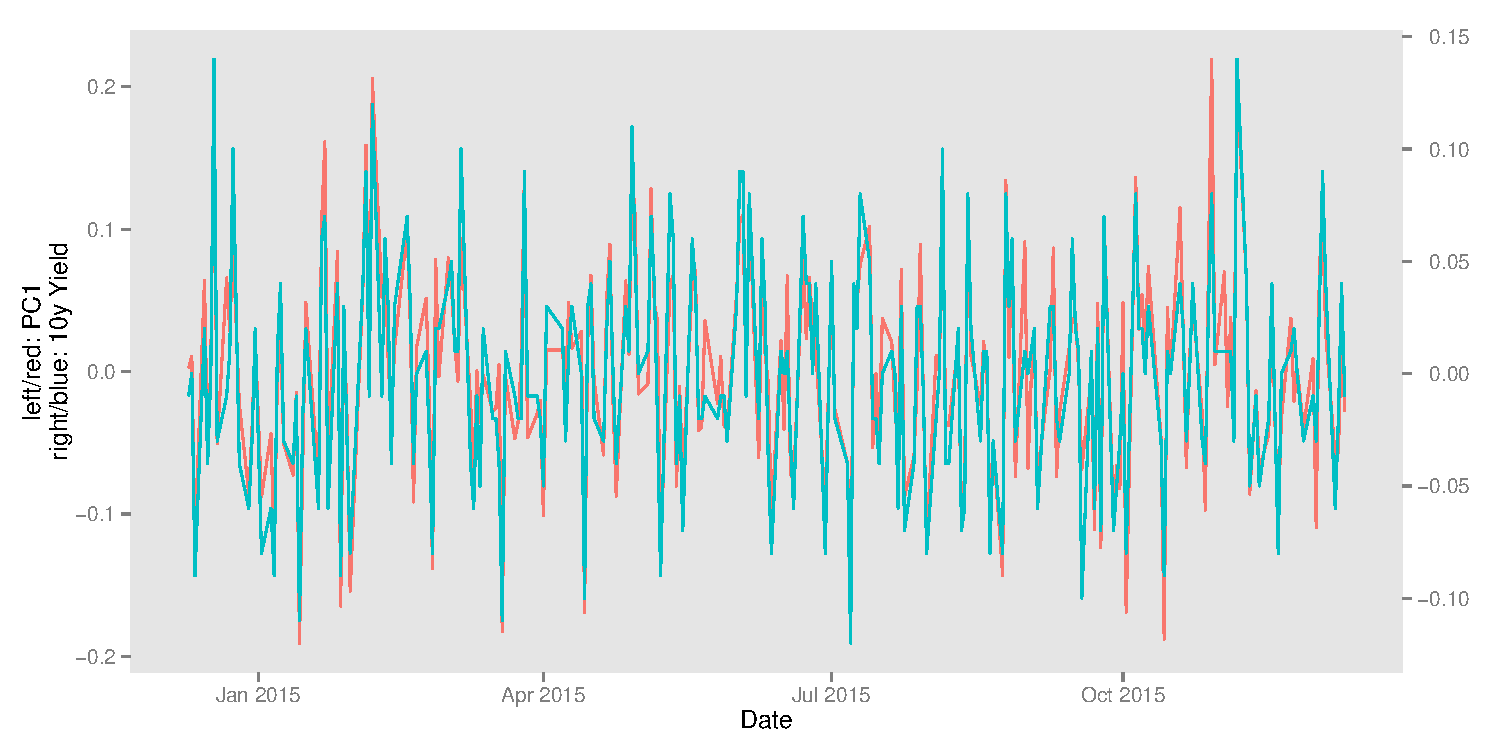
\includegraphics[width=\textwidth]{verify-first.pdf}
\caption{PC1 and returns on 10 year swap rate with correlation coefficient 0.9224358.}
\label{fig:verify-first}
\end{figure}

I plot both the scores of the first principal component and the returns on swap rate for a 10 year IRS in Figure \ref{fig:verify-first} and find that the correlation indeed holds up, and this shows that my interpretation of the principal component holds with correlation coefficient 0.9224358.

\subsection{Second Factor}

To see that the second principal component holds, I use a common curve trade: 10s2s. To see why this represents slope, one can consider the bets I made:

\begin{itemize}
\item Receive fixed for 10 year IRS: if rates go up on the long end, I lose
\item Pay fixed for 2 year IRS: if rates go up in the short end, I gain
\end{itemize}

Hence, I'm making a bet on the slope of the curve. In fact, this bet is a steepener (I profit when the curve steepens). The rate for this trade is constructed as:

\[C_{2, 10} = Y_{0, 10} - Y_{0, 2}\]

where $C$ is the rate for curve trade, $Y$ is the IRS yield.

\begin{figure}[H]
\centering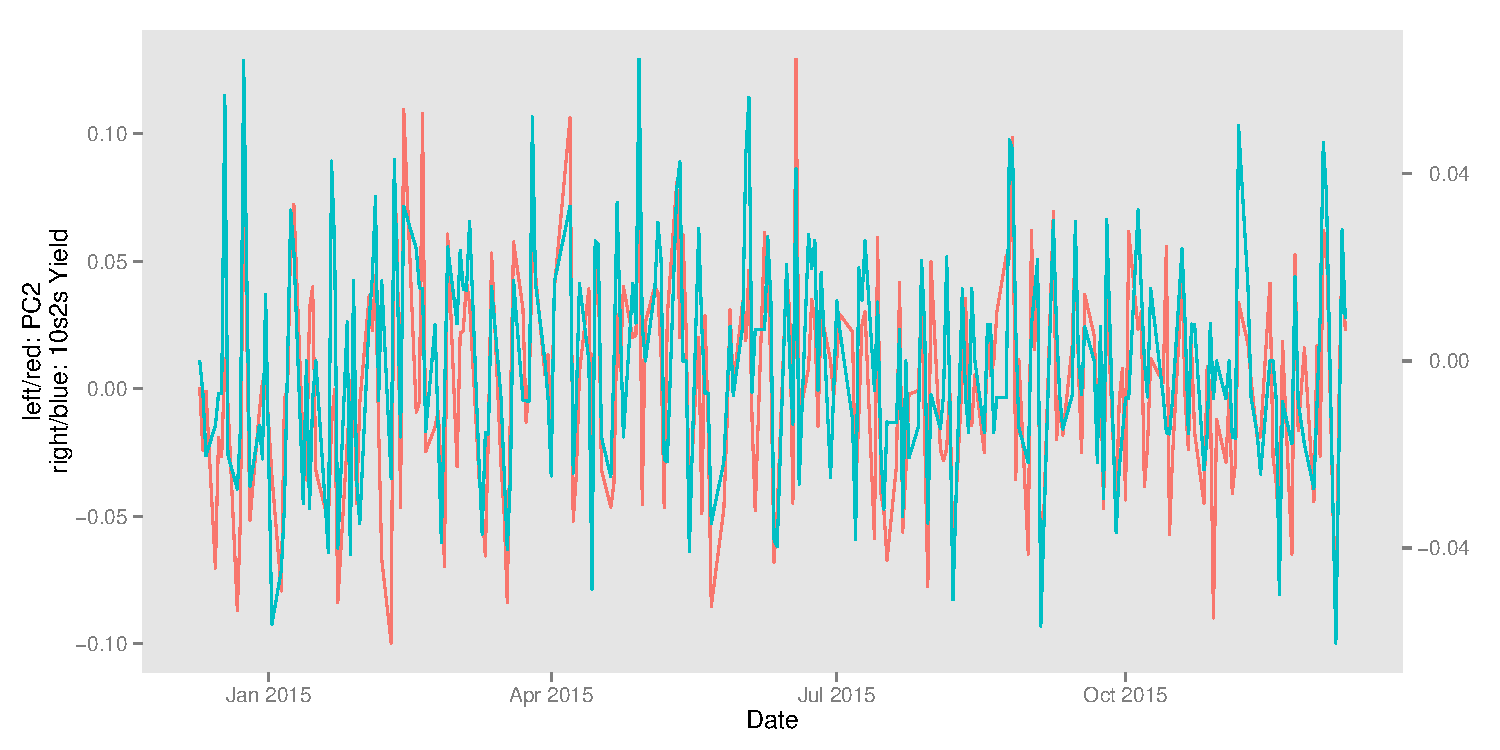
\includegraphics[width=\textwidth]{verify-second.pdf}
\caption{PC2 and returns on 10s2s trade with correlation coefficient 0.6991373.}
\label{fig:verify-second}
\end{figure}

The plot for returns on these yields is shown in Figure \ref{fig:verify-second} The correlation coefficient is 0.6991373.

\subsection{Third Factor}

To see that the third principal component holds, I use another common trade: a butterfly of 2s10s30s. This is essentially:

- Receive fixed on 2 year IRS: I lose if rates go up on the short end
- Pay fixed on two 10 year IRS: I gain if rates go up in the middle end
- Receive fixed on 30 year IRS: I lose if rates go up in the far end

The yield can be constructed as

$$C_{2,10,30} = \left(Y_{0,10} - Y_{0,2}\right) - \left(Y_{0,30} - Y_{0,10}\right)$$

Essentially, I am long two 10 year IRS, and short one 2 year IRS and one 30 year IRS. This can be seen as a bet on curvature. If the rates go up in the middle and go down in the two ends, I profit. Thus this is a curvature bet.

\begin{figure}[H]
\centering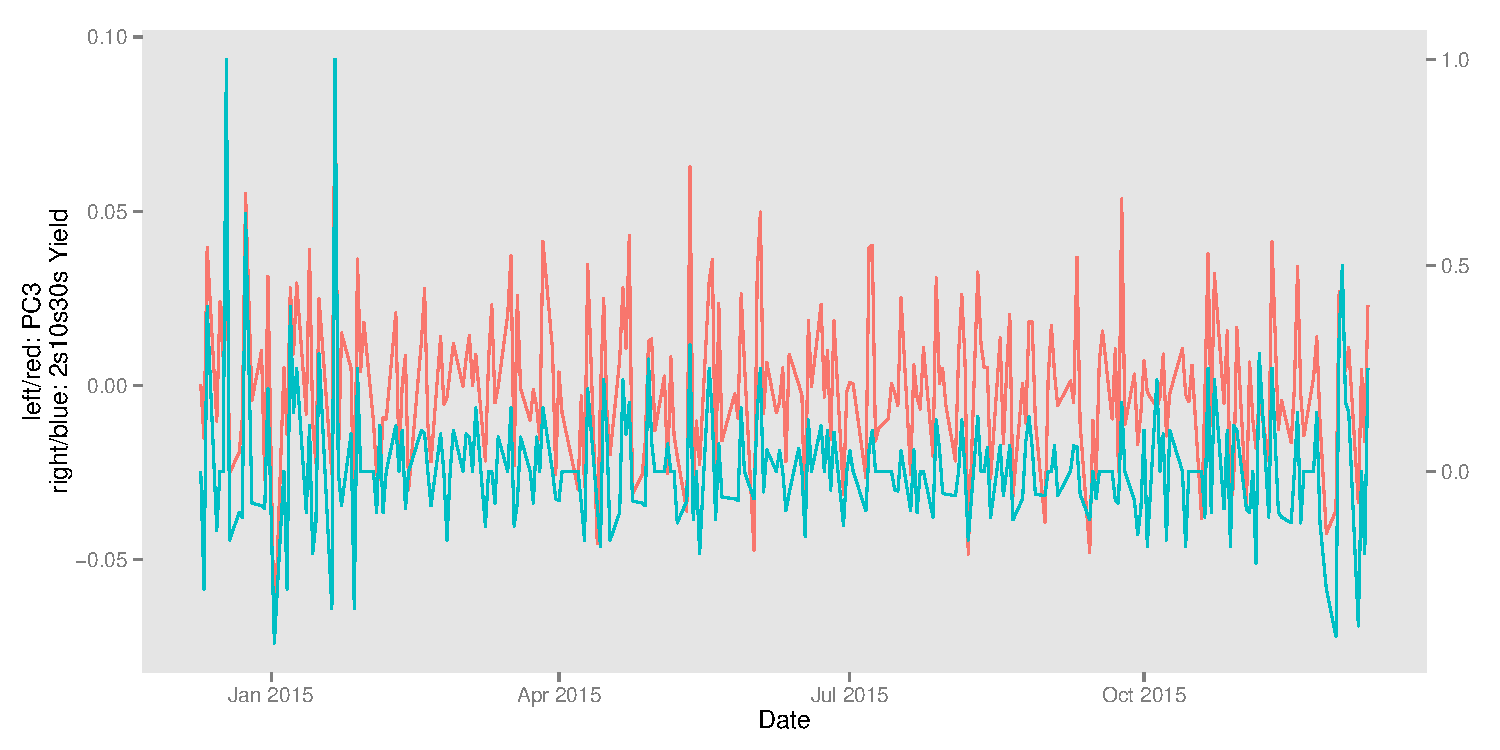
\includegraphics[width=\textwidth]{verify-third.pdf}
\caption{PC3 and returns on 2s10s30s trade with correlation coefficient 0.7499585.}
\label{fig:verify-third}
\end{figure}

The plot is shown in \ref{fig:verify-third}. Again there is a high degree of correlation between this and the yields of a butterfly with the correlation coefficient being 0.7499585, confirming my interpretation of the third principal component.

\chapter{Application to Hedge Ratio Construction}

The applications of this analysis is profound. For starters, it can be used to find a better hedge ratio for two sets of fixed income securities. The typical way to find hedge ratios using duration analysis is to find:

\[N_1 V_1 D_1 = N_2 V_2 D_2\]

where $N_i$ is the number of fixed income instruments of $i$ bought, $V_i$ is the dollar value of the instrument, and $D_i$ is the duration of the instrument. $V_i D_i * 100$ is also known as the Basis Point Value (BPV) of the instrument. Hence, by setting $N_2 = 1$,

\[N_1 = \frac{V_2 D_2}{V_1 D_1}\]

However, this has the critical assumption that a movement shifts the entire yield curve in parallel. In other words, a change that affects yield curve will cause the same amount of shift to the yields of instrument 1 and 2. According to our PCA, this is strictly untrue. As shown in the loadings of the PCA in Table \ref{table:pca-loadings-curve}, different portions of the yield curve move in different extents even in the first order. In fact, the naive duration analysis makes the assumption that all the loadings of PC1 are the same. Hence, a better hedge ratio can easily be constructed using:

\[N_1 V_2 D_1 L_1 = N_2 V_2 D_2 L_2 \]

where $L_i$ is the loading in PC1 for the instrument $i$. This ensures that the extent of shifts of different tenors of the forward curve is captured. Specifically, our analysis using IRS is useful for capturing the movement dynamics of the forward LIBOR curve.

The same analysis can be extended to immunizing PC2 and PC3 risks (even though PC1 itself is already a huge gain eliminating 67.9\% of movements as shown in Table \ref{table:pca-loadings-curve}). This can also be used to immunize portfolios of fixed income instruments on forward rates.

\chapter{Conclusion}

We have demonstrated the usefulness of PCA on IRS, and shown an improvement of naive analysis of IRS rates by using curve rates instead to isolate portions of the forward curve. This analysis is useful in constructing better hedge ratios than naive duration analysis.

\begin{appendices}
All material (code, charts, \LaTeX source files) is available at \url{https://github.com/linanqiu/pca-irs-stat-project}.

\chapter{Interest Rate Swaps}
\begin{aquote}{John C. Hull, Options Futures and Other Derivatives, Chapter 7}
A swap is an over-the-counter agreement between two companies to exchange cash flows in the future. The agreement defines the dates when the cash flows are to be paid and the way in which they are to be calculated. Usually, the calculation of the cash flows involve the future value of an interest rate, an exchange rate, or other market variable. ... The most common type of swap is a "plain vanilla" interest rate swap. In this swap a company agrees to pay cash flows equal to interest at a predetermined fixed rate on a notional principal for a predetermined number of years. In return, it receives interest at a floating rate on the same notional principal for the same period of time.
\end{aquote}

\section{Mechanics of Interest Rate Swaps}

In other words, an interest rate swap (IRS) is an exchange of

\begin{itemize}
\item \textbf{Floating Leg}: a series of coupons paid out at predetermined intervals based on the prevailing interest rate at the beginning of those intervals
\item \textbf{Fixed Leg}: a series of fixed amount coupons paid out at predetermined intervals
\end{itemize}

Hence, it is a swap of a fixed payment and a floating payment flow. The floating leg and the fixed leg coupons are paid as a percent of a notional amount.

\section{LIBOR}
The LIBOR is used as the reference rate for the floating legs in interest rate swaps. LIBOR is the rate that AA rated banks borrow from each other. Over different periods (ranging from say spot to 12 months) the USD LIBOR forward curve is usually above the Treasury Yield curve with mostly the same shape. Hence, the LIBOR forward curve is often used by speculators to speculate on the underlying treasury yield curve (or the ECB rate curve if EUR denominated IRS are used instead).

\section{Bets on Level, Curve, and Curvature}

\subsection{Level Trades}

An IRS is an instrument to bet on the entire forward curve from spot rate to the year of maturity. A "5y" allows us to bet on the entire curve up to the 5 year point.

In terms of directions:

\begin{itemize}
\item If I pay fixed (receive float), when the yield curve goes up, I profit (since I'm paying less than I would have).
\item If I receive fixed (pay float), when the yield curve goes up, I lose (since I'm paying more).
\end{itemize}

\subsection{Curve Trades}

Then, one can imagine a trade where:

\begin{itemize}
\item I pay fixed (receive float) on one 2 year IRS: I profit from the yield curve going up at the short end
\item I pay float (receive fixed) on one 10 year IRS: I profit from the yield curve going down at the long end
\end{itemize}

The fixed payments from now to year 2 cancel each other out, just as the floating payments. Hence, I am betting on the curve from year 2 to year 10. In other words, I am betting on a specific section of the curve, not just from today till the end of the curve. In particular, I am betting that the section of the curve \emph{flattens} (going up at the short end and going down at the long end). There's an important caveat to this: \textbf{I do not hold this trade to maturity.} Otherwise, this would cease to be a curve trade. The 2 year would expire and I would be left with one outstanding swap, making this a normal directional bet.

\subsection{Butterfly Trades}

Butterfly trades benefit from differing movements in 3 instruments. Imagine this trade:

\begin{itemize}
\item I pay fixed (receive float) on 2 year IRS: I profit from yield curve going up at the short end
\item I receive float (pay fixed) on two 10 year IRS: I profit from the yield curve going down at the middle end
\item I pay fixed (receive float) on 30 year IRS: I profit from the yield curve going up at the long end
\end{itemize}

I essentially bet on the curvature of the curve. An imaginative trader gave this trade the name, presumably because of the symmetric direction.

\chapter{Data}

\section{IRS Rates}

\begin{figure}[H]
\centering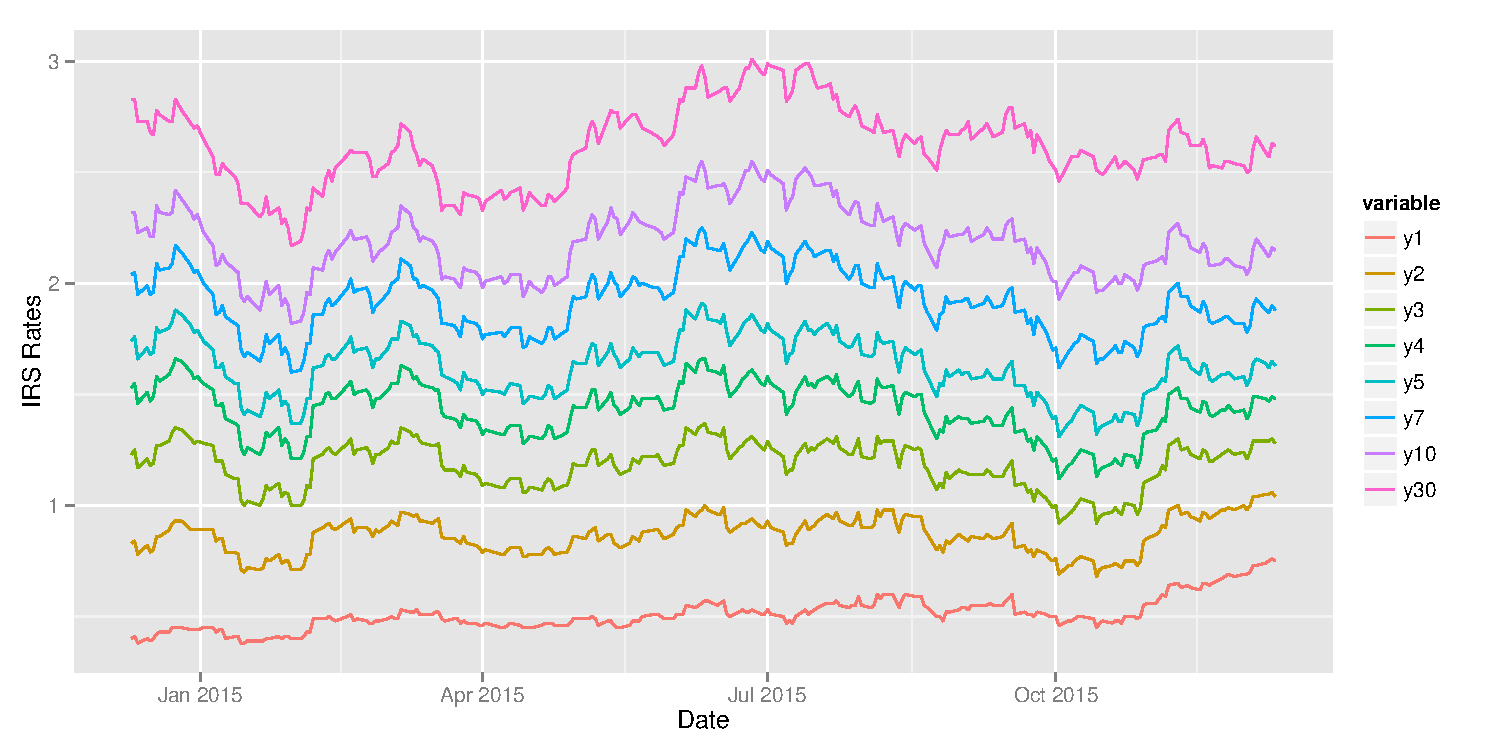
\includegraphics[width=\textwidth]{descriptive-rates.pdf}
\caption{IRS Swap Rates}
\label{fig:descriptive-rates}
\end{figure}

\begin{figure}[H]
\centering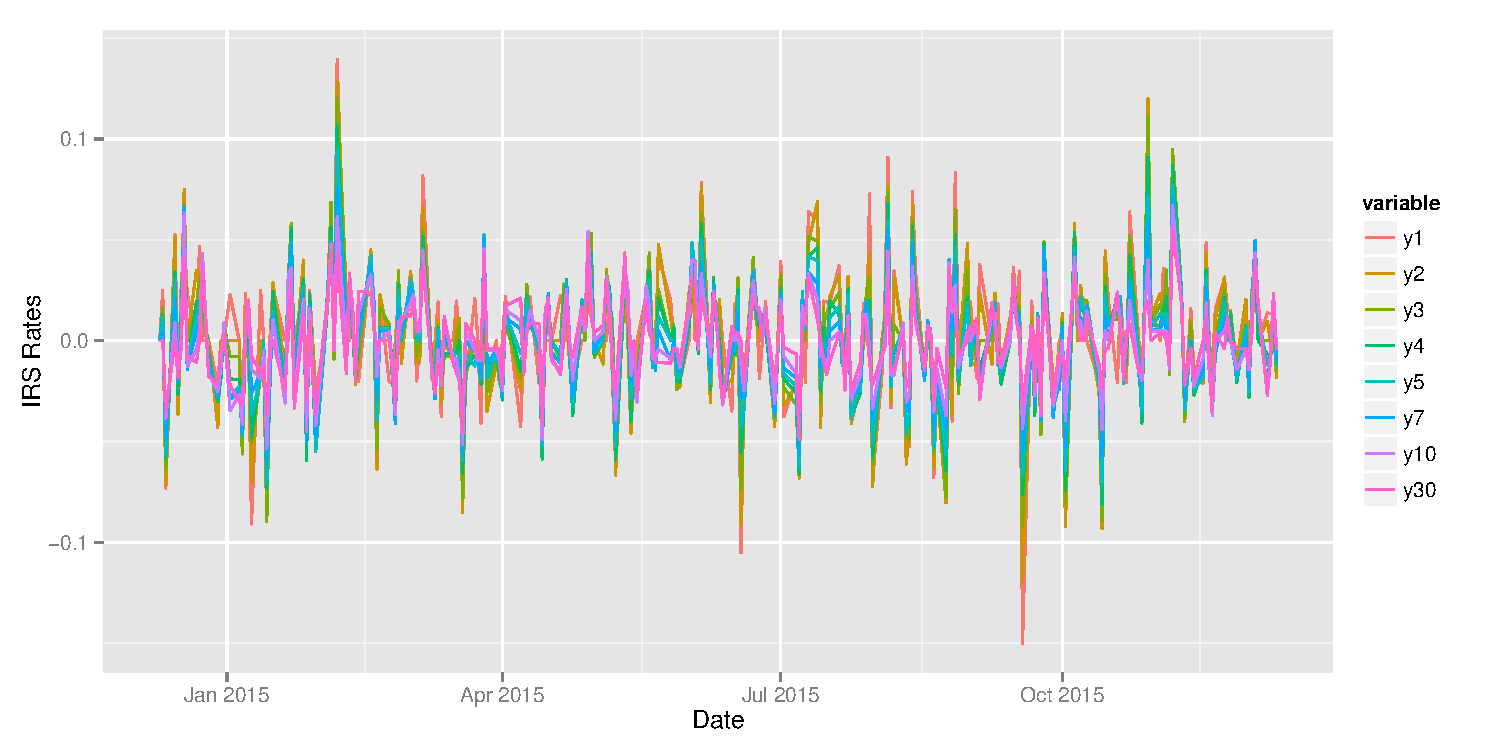
\includegraphics[width=\textwidth]{descriptive-rates-returns.pdf}
\caption{Returns on IRS Swap Rates}
\label{fig:descriptive-rates-returns}
\end{figure}

\begin{figure}[H]
\centering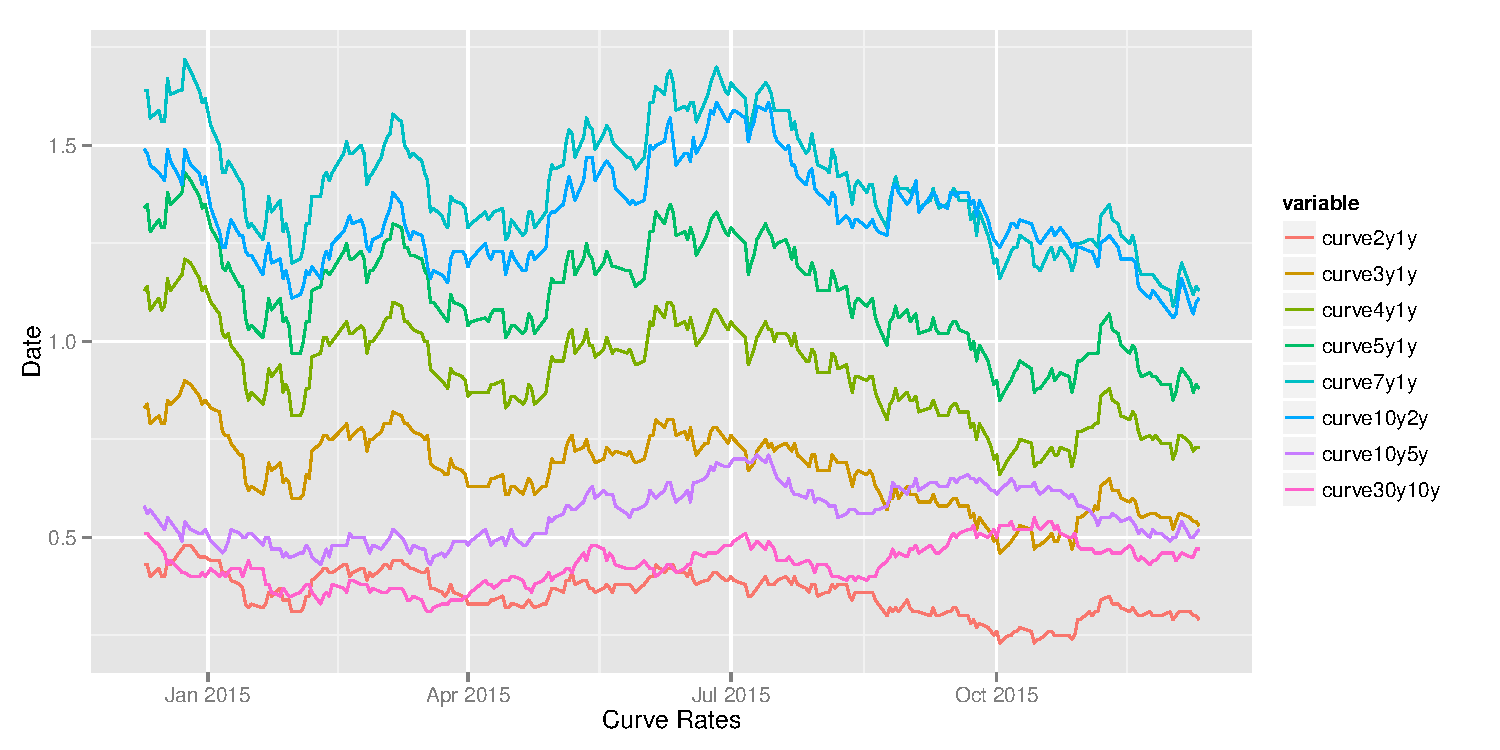
\includegraphics[width=\textwidth]{descriptive-curve-rates.pdf}
\caption{IRS Curve Swap Rates}
\label{fig:descriptive-curve-rates}
\end{figure}

\begin{figure}[H]
\centering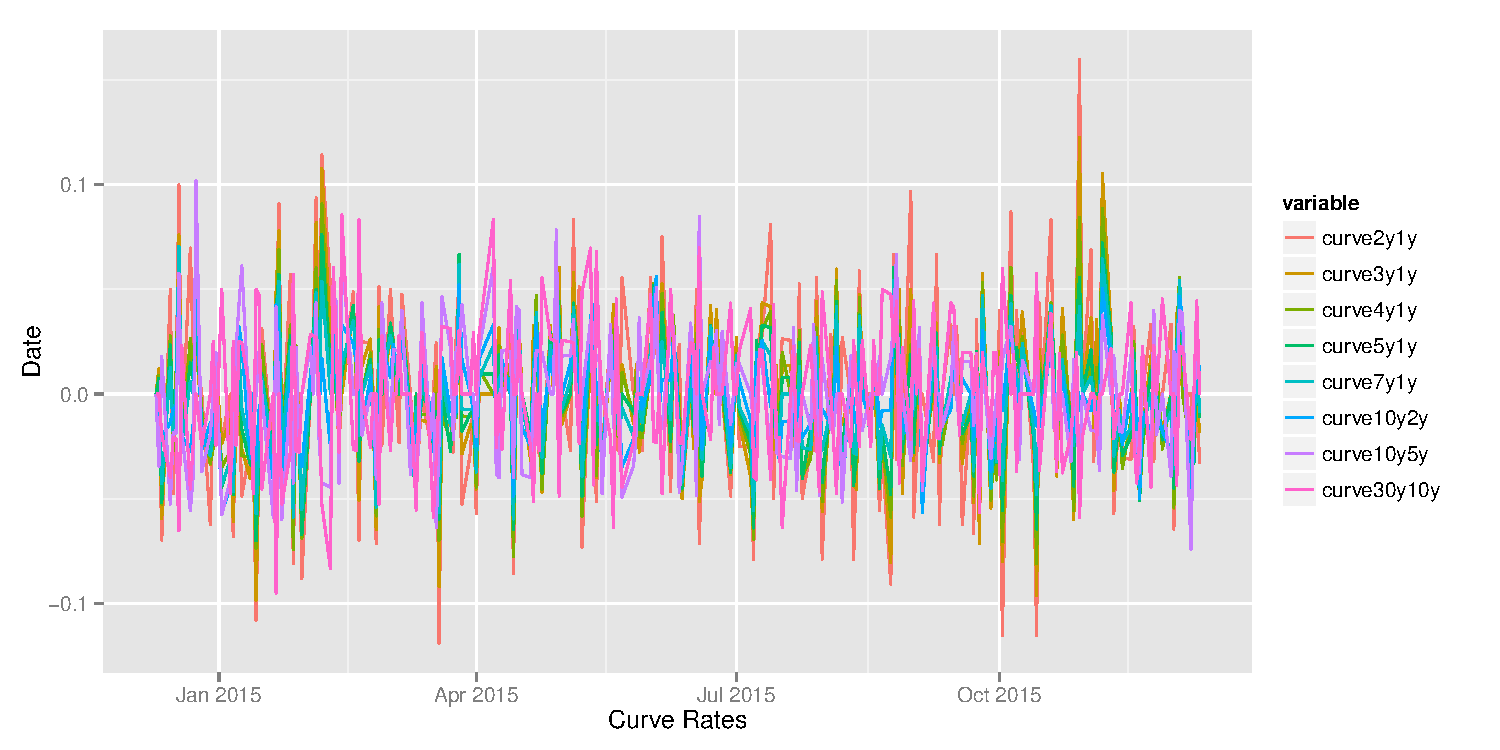
\includegraphics[width=\textwidth]{descriptive-curve-rates-returns.pdf}
\caption{Returns on IRS Curve Swap Rates}
\label{fig:descriptive-curve-rates-returns}
\end{figure}

\section{Autocorrelation}

\begin{figure}[H]
\centering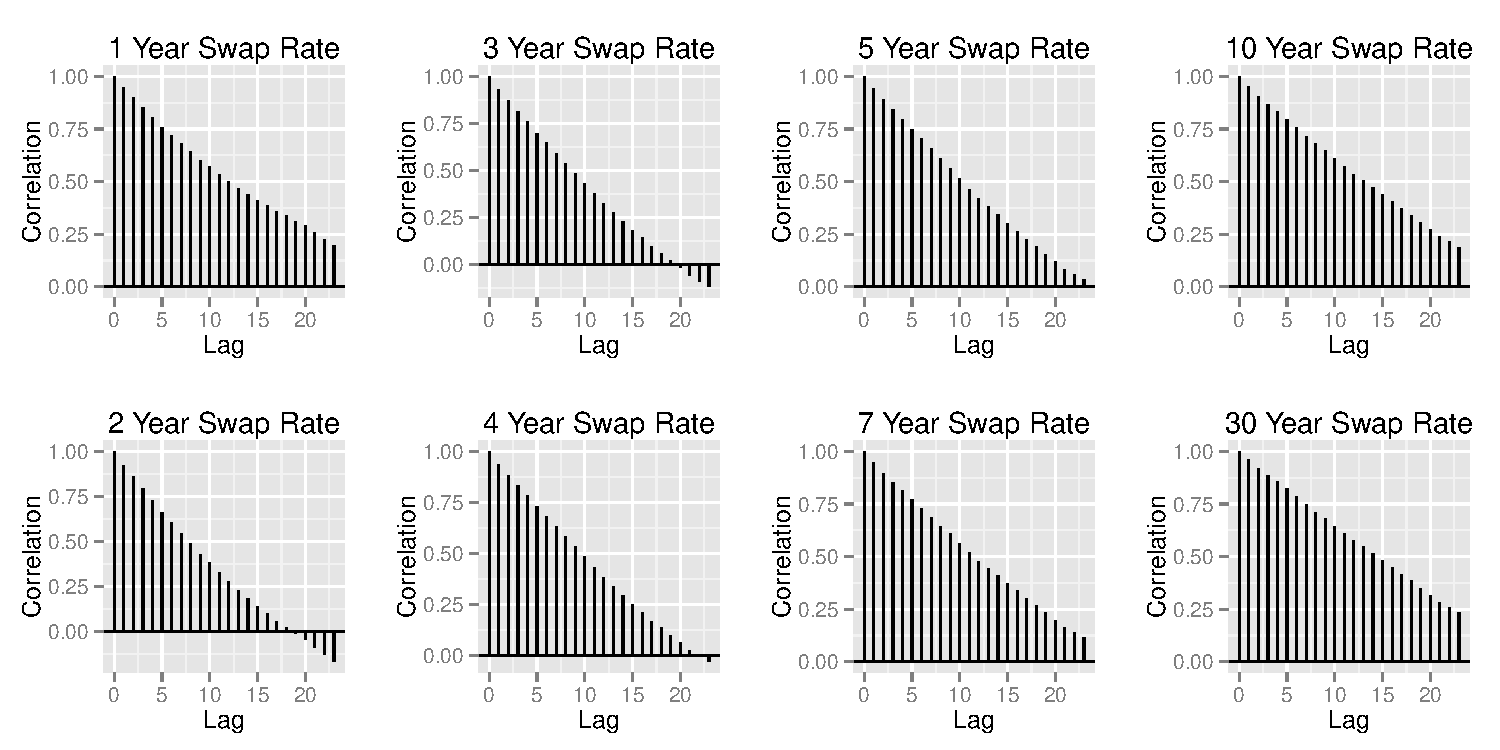
\includegraphics[width=\textwidth]{acf-yields.pdf}
\caption{Autocorrelation of yield levels. Yield levels are highly autocorrelated.}
\label{fig:acf-yields}
\end{figure}

\begin{figure}[H]
\centering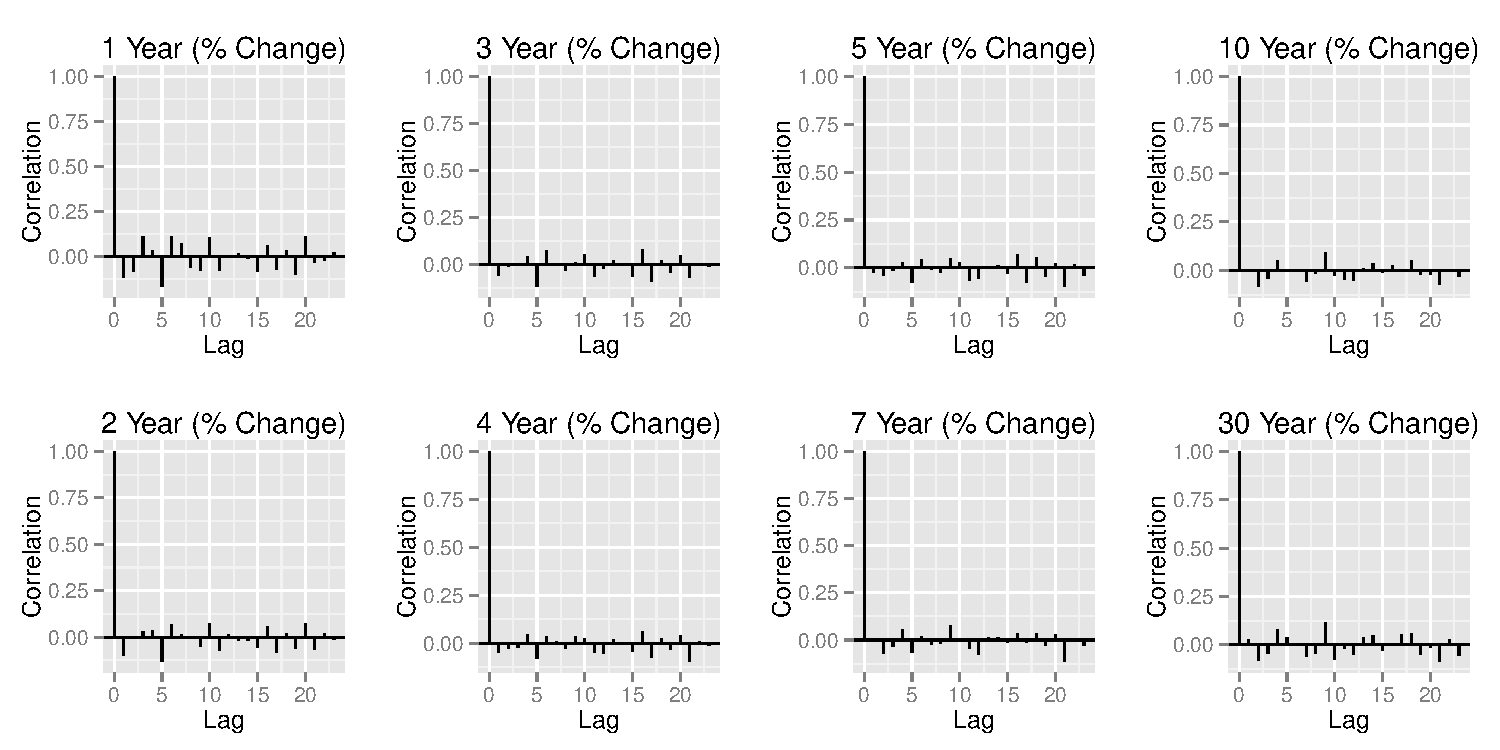
\includegraphics[width=\textwidth]{acf-yields-returns.pdf}
\caption{Autocorrelation of yield percentage changes, showing minimal autocorrelation.}
\label{fig:acf-yields-returns}
\end{figure}

\begin{figure}[H]
\centering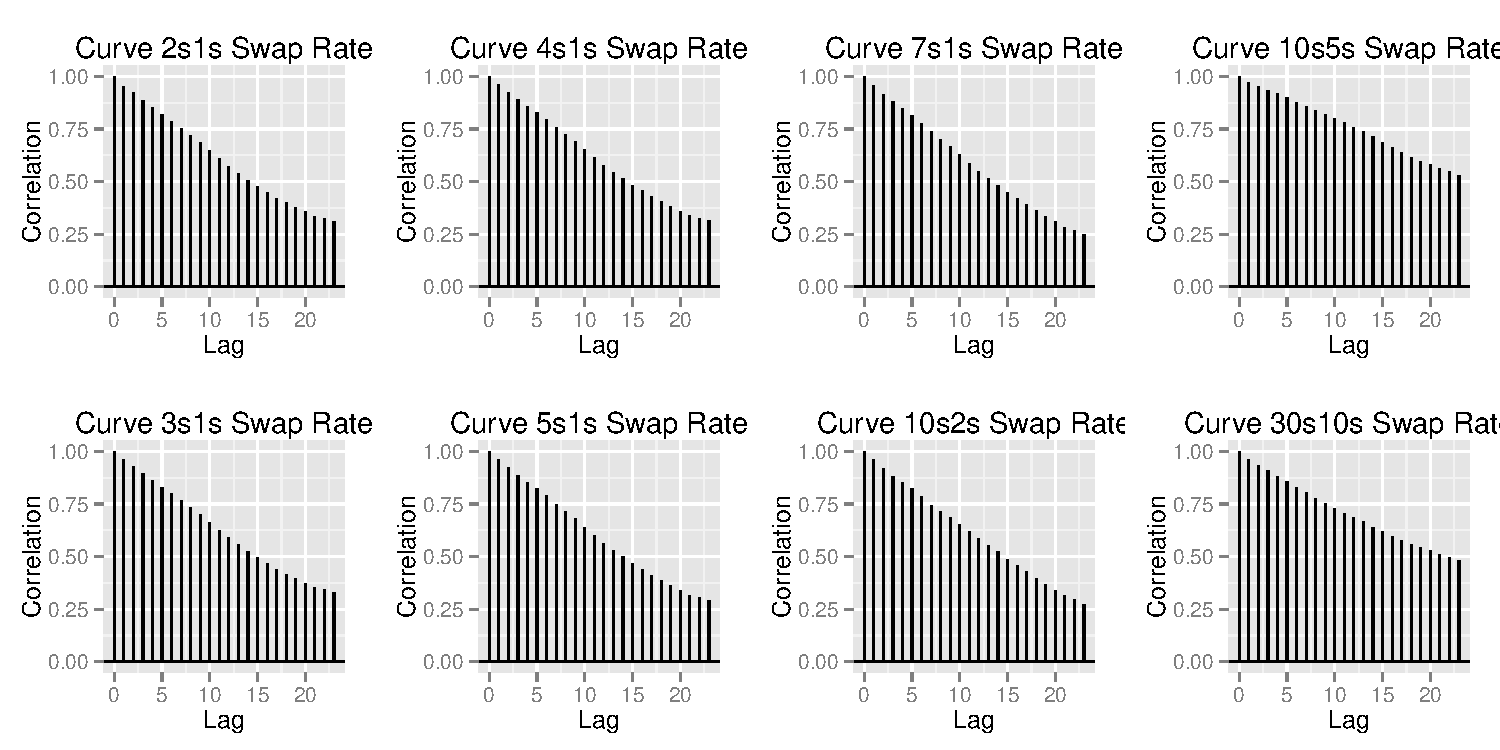
\includegraphics[width=\textwidth]{acf-curve.pdf}
\caption{Autocorrelation of curve rate levels. Yield levels are highly autocorrelated.}
\label{fig:acf-curve}
\end{figure}

\begin{figure}[H]
\centering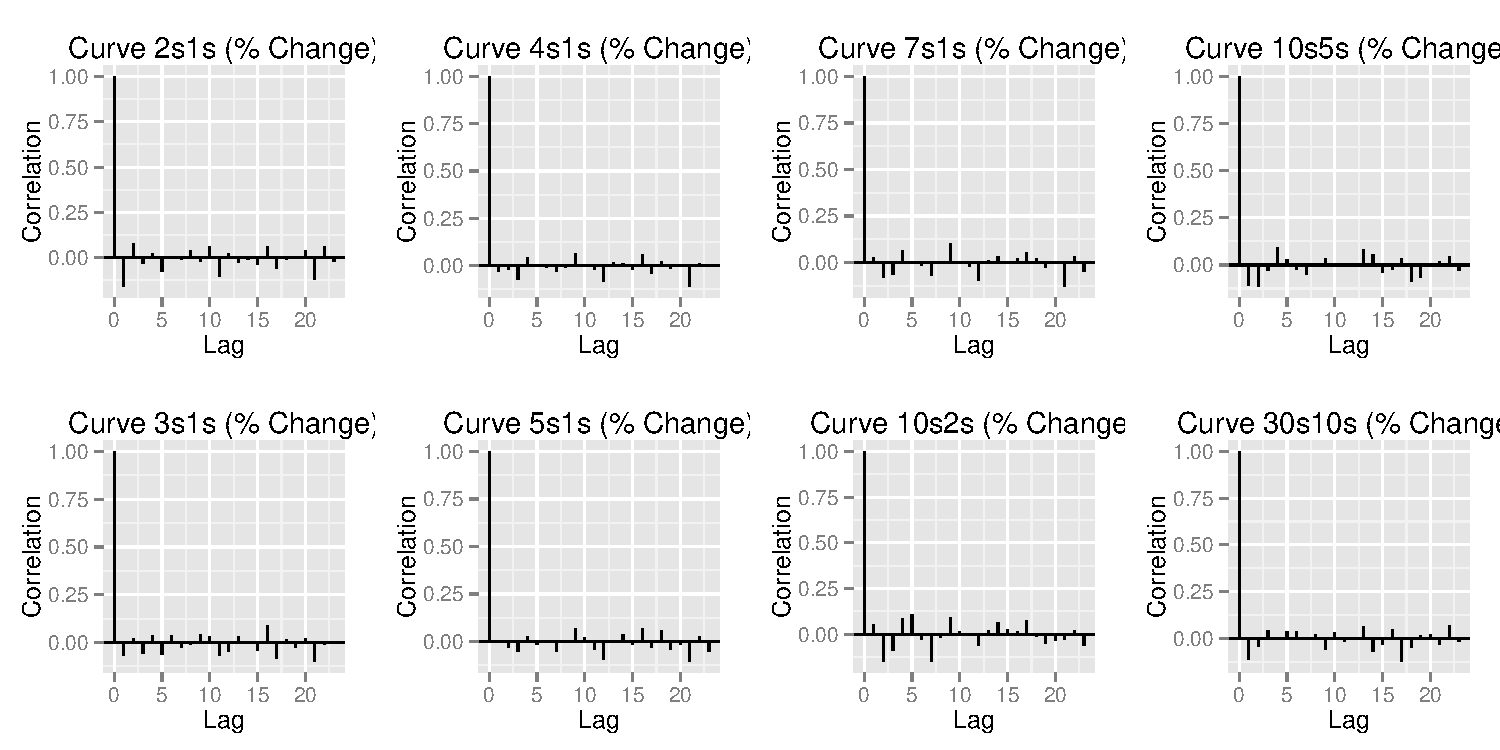
\includegraphics[width=\textwidth]{acf-curve-returns.pdf}
\caption{Autocorrelation of curve rate percentage changes, showing minimal autocorrelation.}
\label{fig:acf-curve-returns}
\end{figure}

\begin{landscape}
\chapter{PCA on IRS Level Trades}
\section{Summary of PCA Results}

\begin{figure}[H]
\begin{lstlisting}
Importance of components:
                           Comp.1     Comp.2      Comp.3      Comp.4      Comp.5      Comp.6      Comp.7       Comp.8
Standard deviation     0.07686063 0.02203250 0.009395619 0.005489417 0.003737261 0.002861156 0.002560305 0.0021638991
Proportion of Variance 0.90263501 0.07417061 0.013488234 0.004604227 0.002134082 0.001250799 0.001001585 0.0007154484
Cumulative Proportion  0.90263501 0.97680562 0.990293858 0.994898085 0.997032168 0.998282967 0.999284552 1.0000000000
\end{lstlisting}
\caption{Proportion of Explained Variance for each PC}
\label{fig:verbatim-vanilla}
\end{figure}

\end{landscape}

\section{PCA Loadings}

\begin{table}[ht]
\centering
\begin{tabu}{rrrrrrrrr}
  \toprule
 & Comp.1 & Comp.2 & Comp.3 & Comp.4 & Comp.5 & Comp.6 & Comp.7 & Comp.8 \\ 
  \midrule
y1 & -0.40 & 0.61 & 0.66 & -0.15 & 0.03 & -0.02 & 0.00 & 0.00 \\ 
  y2 & -0.44 & 0.29 & -0.38 & 0.73 & 0.19 & 0.01 & -0.07 & -0.03 \\ 
  y3 & -0.41 & 0.07 & -0.34 & -0.24 & -0.77 & -0.22 & 0.05 & -0.01 \\ 
  y4 & -0.38 & -0.10 & -0.22 & -0.39 & 0.20 & 0.74 & -0.19 & -0.13 \\ 
  y5 & -0.35 & -0.19 & -0.12 & -0.24 & 0.42 & -0.29 & 0.71 & 0.07 \\ 
  y7 & -0.31 & -0.32 & 0.08 & -0.07 & 0.17 & -0.29 & -0.52 & 0.64 \\ 
  y10 & -0.26 & -0.41 & 0.23 & 0.06 & 0.06 & -0.30 & -0.27 & -0.73 \\ 
  y30 & -0.20 & -0.46 & 0.42 & 0.41 & -0.34 & 0.38 & 0.33 & 0.20 \\ 
   \bottomrule
\end{tabu}
\caption{Loadings of PCA on IRS Level Trades}
\label{table:pca-loadings-level}
\end{table}

\begin{figure}[H]
\centering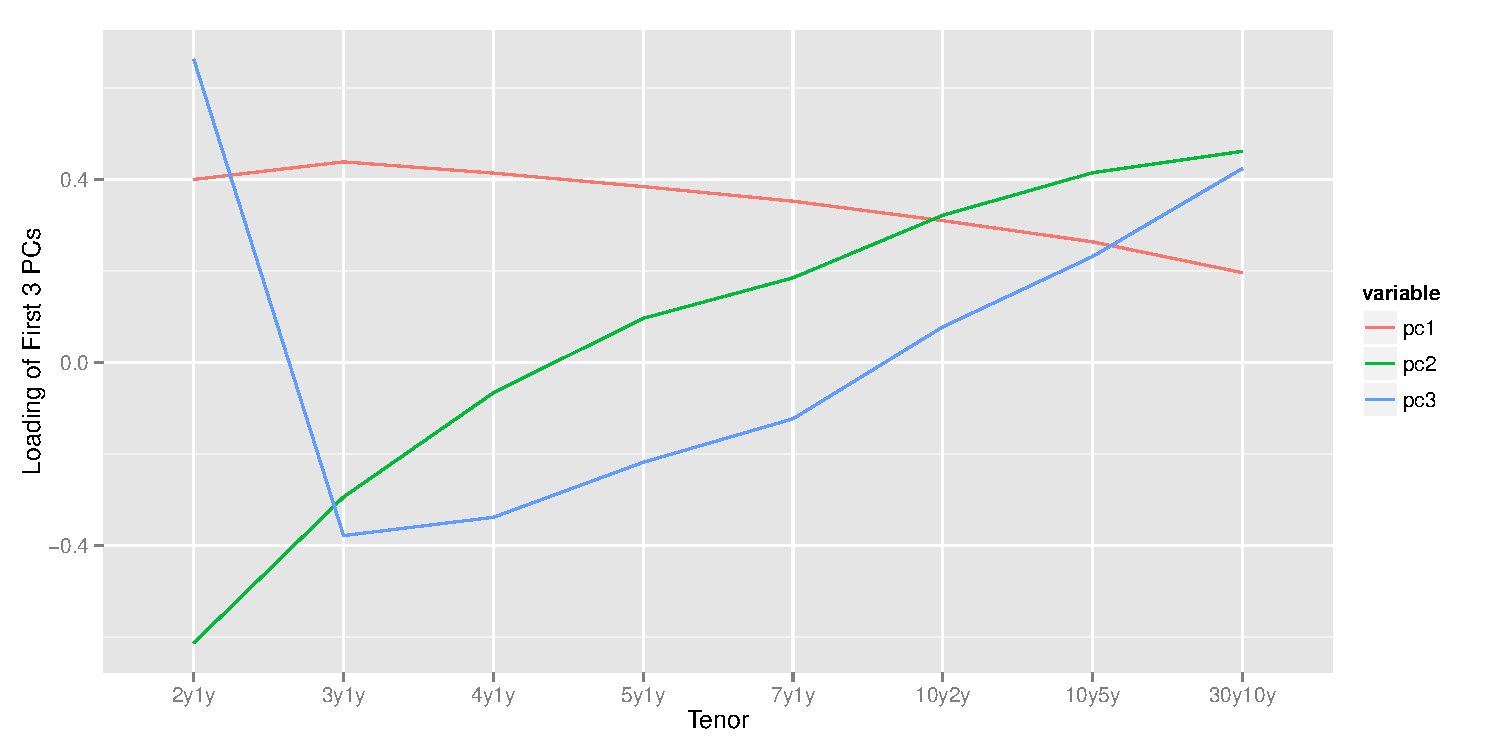
\includegraphics[width=\textwidth]{pca-loadings-vanilla.pdf}
\caption{Loadings of principal components for IRS Level Trades for each tenor}
\label{fig:pca-loadings-vanilla}
\end{figure}

\section{PCA Scores}

\begin{figure}[H]
\centering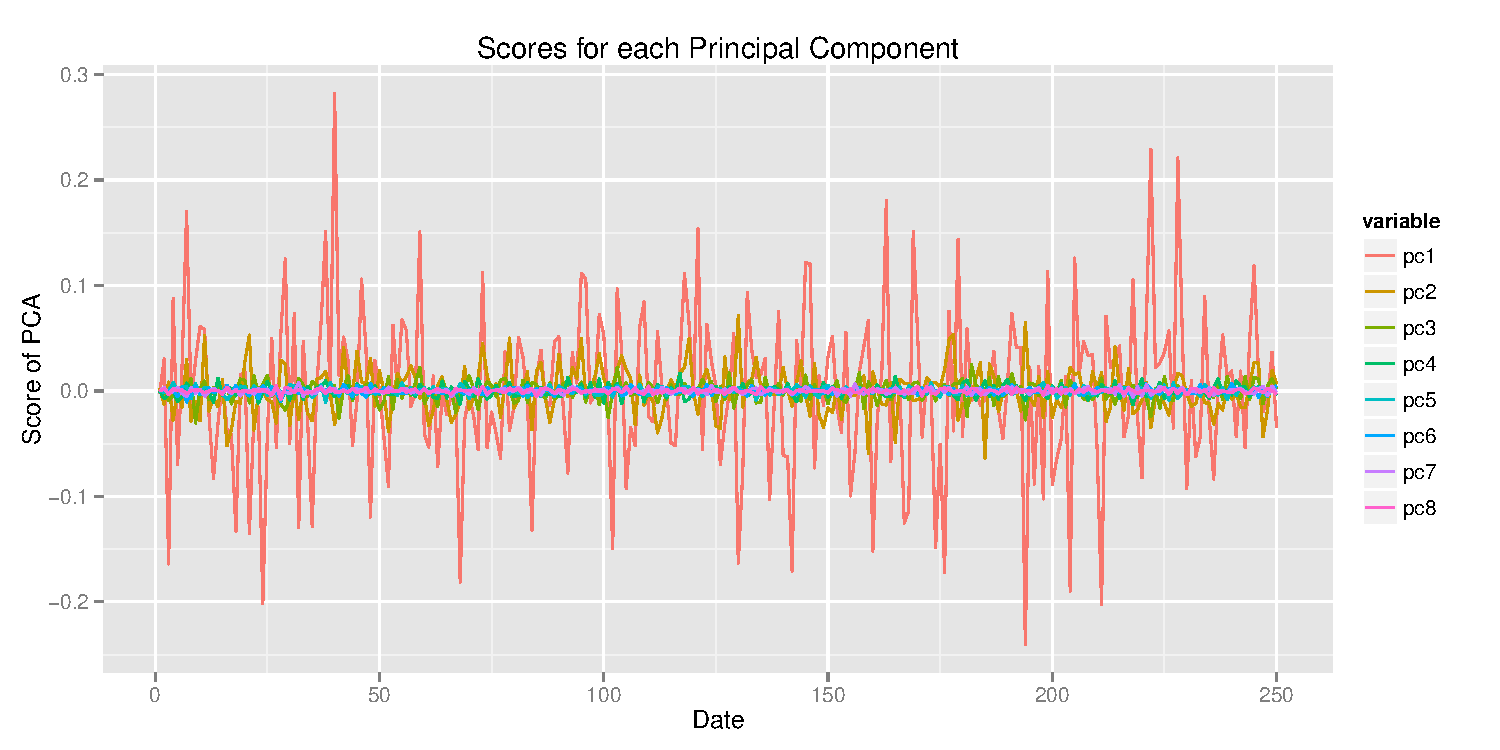
\includegraphics[width=\textwidth]{pca-scores-vanilla.pdf}
\caption{Scores of principal components for IRS Level Trades}
\label{fig:pca-scores-vanilla}
\end{figure}

\begin{landscape}
\chapter{PCA on IRS Curve Trades}
\section{Summary of PCA Results}

\begin{figure}[H]
\begin{lstlisting}
Importance of components:
                           Comp.1     Comp.2     Comp.3     Comp.4      Comp.5      Comp.6      Comp.7       Comp.8
Standard deviation     0.07444059 0.04272714 0.02279233 0.01345661 0.007430373 0.004724775 0.003359157 0.0007782348
Proportion of Variance 0.67934275 0.22380865 0.06368644 0.02219937 0.006768471 0.002736727 0.001383343 0.0000742490
Cumulative Proportion  0.67934275 0.90315140 0.96683783 0.98903721 0.995805681 0.998542408 0.999925751 1.0000000000
\end{lstlisting}
\caption{Proportion of Explained Variance for each PC}
\label{fig:verbatim-curve}
\end{figure}

\end{landscape}

\section{PCA Loadings}

\begin{table}[ht]
\centering
\begin{tabu}{rrrrrrrrr}
  \toprule
 & Comp.1 & Comp.2 & Comp.3 & Comp.4 & Comp.5 & Comp.6 & Comp.7 & Comp.8 \\ 
  \midrule
curve2y1y & -0.54 & 0.23 & 0.37 & 0.64 & 0.25 & 0.03 & -0.07 & 0.19 \\ 
  curve3y1y & -0.47 & 0.07 & 0.06 & -0.17 & -0.81 & 0.30 & -0.03 & 0.01 \\ 
  curve4y1y & -0.42 & -0.03 & -0.03 & -0.29 & -0.02 & -0.86 & -0.04 & 0.01 \\ 
  curve5y1y & -0.38 & -0.07 & -0.04 & -0.30 & 0.38 & 0.29 & -0.41 & -0.60 \\ 
  curve7y1y & -0.33 & -0.19 & -0.08 & -0.16 & 0.24 & 0.18 & 0.86 & -0.04 \\ 
  curve10y2y & -0.20 & -0.39 & -0.29 & -0.19 & 0.20 & 0.21 & -0.29 & 0.72 \\ 
  curve10y5y & -0.08 & -0.63 & -0.38 & 0.56 & -0.20 & -0.11 & -0.03 & -0.29 \\ 
  curve30y10y & 0.12 & -0.59 & 0.78 & -0.13 & -0.03 & -0.02 & -0.02 & 0.00 \\ 
   \bottomrule
\end{tabu}
\caption{Loadings of PCA on IRS Curve Trades}
\label{table:pca-loadings-curve}
\end{table}

\begin{figure}[H]
\centering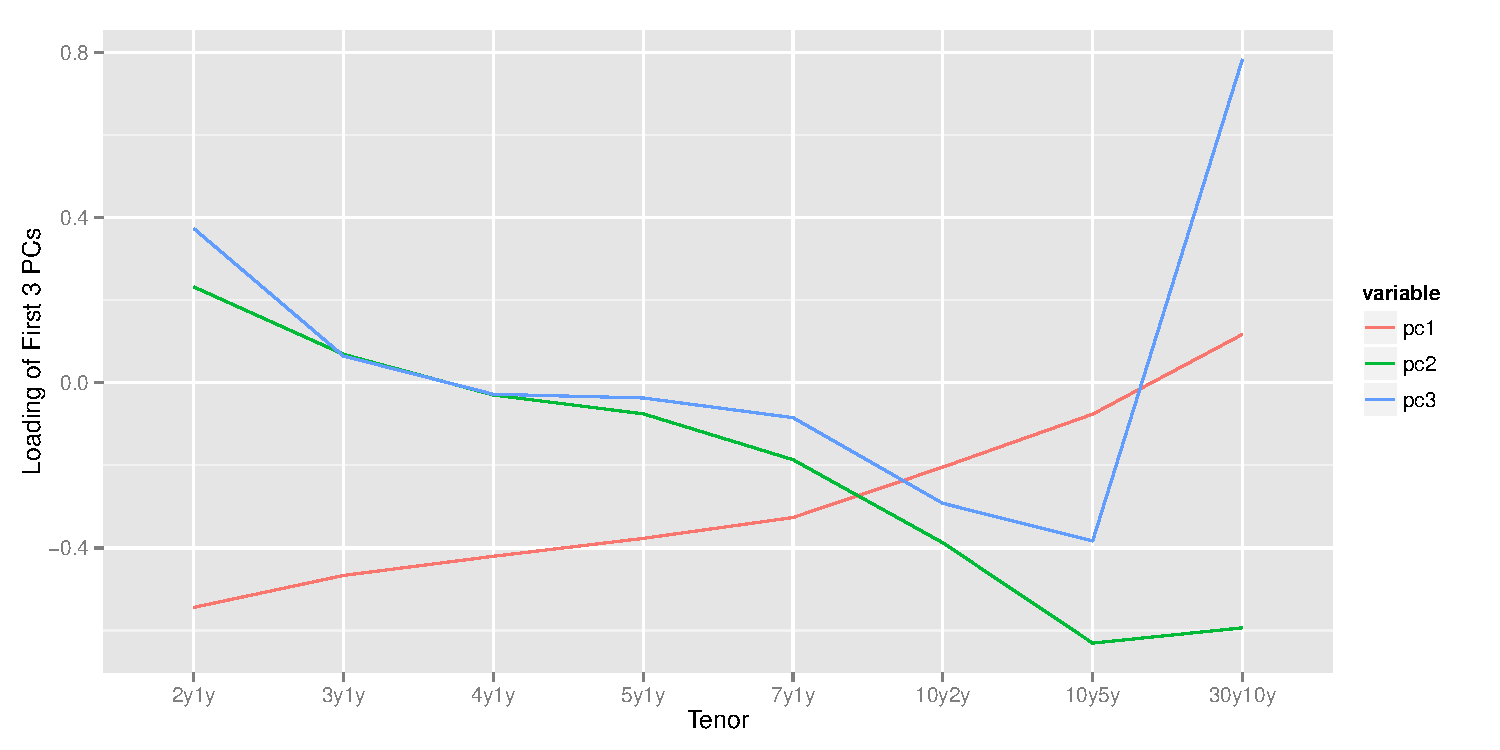
\includegraphics[width=\textwidth]{pca-loadings-curve.pdf}
\caption{Loadings of principal components for IRS Curve Trades for each tenor}
\label{fig:pca-loadings-curve}
\end{figure}

\section{PCA Scores}

\begin{figure}[H]
\centering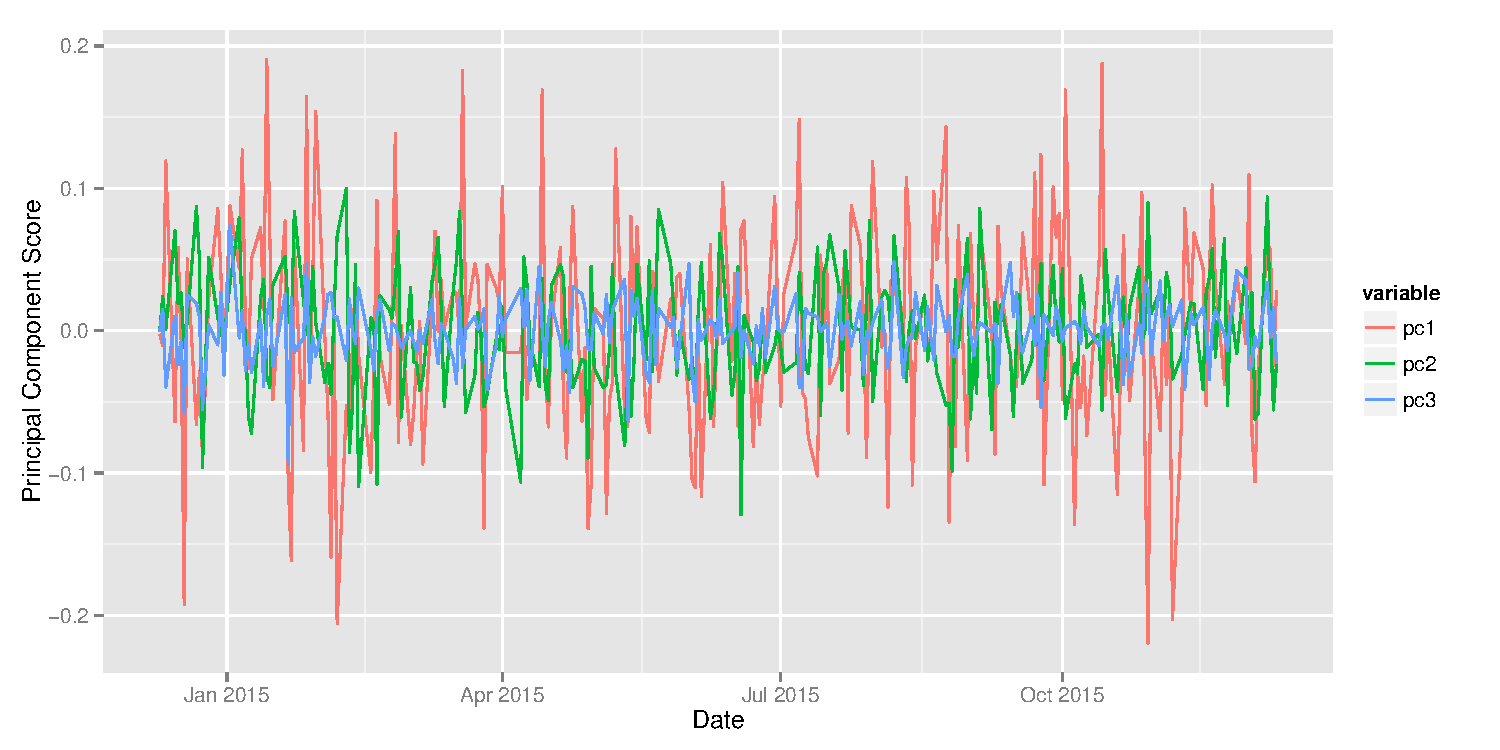
\includegraphics[width=\textwidth]{pca-scores-curve.pdf}
\caption{Scores of principal components for IRS Curve Trades}
\label{fig:pca-scores-curve}
\end{figure}
\end{appendices}

\end{document}
